\graphicspath{{./Lecture3/}}
\section{Singular Points}

Singular points are divided into two classes:

\begin{itemize}
    \item Regular singular points, where we use the Frobenius series solution
    \item Irregular singular points, which are beyond the scope of the course
\end{itemize}

If we are to look at the ODE $P(x) y'' + Q(x) y' + R(x) y = 0$, and define the point $x_0$ as a singular point, we have the following:

The Cauchy-Euler equation is 

\begin{equation}
\label{Cauchy-Euler}
    (x - x_0)^2 + \alpha (x - x_0) y' + \beta y = 0
\end{equation}

We know that $y = (x - x_0)^r$ (As an example). 

How do we make $P(x) y'' + Q(x) y' + R(x) y = 0$ look like( \ref{Cauchy-Euler})?

If we multiply with $(x - x_0)^2$ and divide by $P(x)$, we may get something similar to the Cauchy-Euler. 

Then, we get something like this:
\begin{equation}
    (x - x_0)^2 y'' + \left\{ \frac{Q(x)}{P(x)} (x - x_0) \right\} (x - x_0) y' + \left\{ \frac{R(x)}{P(x)} (x - x_0)^2 \right\} y = 0
\end{equation}


Now, if $\frac{Q(x)}{P(x)}(x - x_0)$ and $\frac{R(x)}{P(x)} (x - x_0)^2$ are analytic at $x = x_0$, then the singularity is not worse than the singularity in the Cauchy-Euler equation (\ref{Cauchy-Euler}), \textbf{and} $x_0$ is a "regular singular point". Otherwise, $x_0$ is an "irregular singular point". 

If we start to write the Taylor series for (?),

$\frac{Q(x)}{P(x)} (x - x_0) = p_0 + p_1 (x - x_0) + ...$

$\frac{R(x)}{P(x)} (x - x_0)^2 = q_0 + q_1 (x - x_0) + ...$

Being analytic means that we need to be able to write the series. 

An example of a singular point:

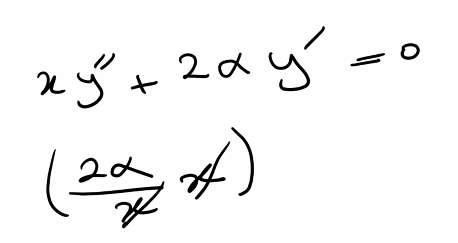
\includegraphics[width = 0.6 \textwidth]{image1.png}

Here, $x = 0$ is a singular point. (We re-wrote the first equation as the second equation, I believe)

\hfill \break

As $x \longrightarrow x_0$, our ODE becomes: $(x - x_0)^2 y'' + p_0 (x - x_0) y' + q_0 y = 0$

The corresponding Cauchy-Euler equation solution: $y = (x - x_0)^r$. We need to have finite $p_0$ and $q_0$. If $p_0$ and $q_0$ are both finite, then $x_0$ is a regular singular point. Otherwise, it is an irregular singular point. 

For regular singular points, the solution we are going to write: 

$$\underbrace{y(x) = (x - x_0)^r}_{*} \underbrace{\sum_{n = 0}^{\infty} a_n (x - x_0)^n}_{\text{Correction}}$$

*: The singular part of the solution to the corresponding Cauchy-Euler. 

\subsection{Example}

$$x(1+x^2) y'' + 2xy' + (1+x^2) y = 0$$. 

Classify singular points. Here, $p(x) = x(1+x)^2$, $Q(x) = 2x$, and $R(x) = 1+x^2$. Singular points: $\left\{ \begin{matrix} x = 0 \\ x = \pm i \end{matrix} \right.$ We need $p(x_0) = 0$ (Take a look at the left hand side if you don't understand!). 

Classify them:

$\left\{ \begin{matrix} \lim_{x \rightarrow x_0} \frac{Q(x)}{P(x)} (x - x_0) = p_0 \\ \lim_{x \rightarrow x_0} \frac{R(x)}{P(x)} (x - x_0)^2 = q_0 \end{matrix} \right.$

For $x_0 = 0$, we have $\lim_{x \to 0} \frac{2x}{x(1+x^2)} x = 0 = p_0$

$\lim_{x \to 0} \frac{1+x^2}{x(1+x^2)} x^2 = 0 = q_0$

\hfill \break 

Now for $x_0 = i$:

$\lim_{x \to i} \frac{2x}{x (1+x^2)} (x - i) = \lim_{x \to i} \frac{2(x-i}{(x-i)(x+i)} = \frac{1}{i} = p_0$

$\lim_{x \to i} \frac{1+x^2}{x(1+x^2)} (x-i)^2 = 0 = q_0$

We see that because both $p_0$ and $q_0$ are finite, $x = i$ is also a regular singular point. 

Try for $x = -i$:

$\lim_{x \to -i} \frac{2x}{x (1+x^2)} (x+i)$

$\lim_{x \to -i} \frac{1+x^2}{x(1+x^2)} (x+i)^2$

yeah uhhhh.... review how to calculate limits. 

When we calculate $x_0 = -i$, we get: $p_0 = -\frac{1}{i}$, and $q_0 = 0$. Hence, $x_0 = -i$ is also a regular singular point. 

\section{Radius of Convergence}

The radius of convergence of the series solution is at least equal to the distance from the $x_0$ to the nearest singular point. In the example that we solved:

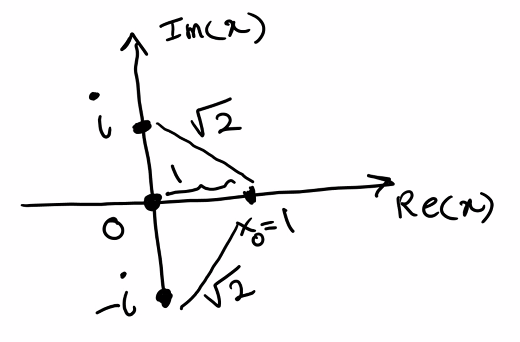
\includegraphics[width = 0.7 \textwidth]{image2.png}

$y(x) = \sum_{n = 0}^{\infty} a_n (x-1)^n$

$\rho = 1$ is the lower bound estimate. $\rho$ is the radius of convergence. Imagine a circle of radius 1 (as it's the distance to the closest singular point)

\subsubsection{An Example}

$$x^2 y'' + \alpha x y' + \beta y = 0$$

$r_1, r_2$ are two positive roots

$$y = C_1 x^{r_1} + C_2 x^{r_2}$$

$x_0 = 0$ is a singular point

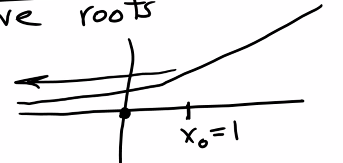
\includegraphics[width = 0.4 \textwidth]{image3.png}

Radius of convergence is infinite. This is a rare case. 

\section{Frobenius Series}

EX: 

$$ 6x^2 (1+x) y'' + 5xy' - y = 0$$

$P(x) = 6x^2 (1+x)$, $Q(x) = 5x$, $R(x) = -1$

Singular points are $x = 0$ and $x = -1$. 

For $x = 0$, let's find if it's irregular or regular:

$\lim_{x \to 0} \frac{Q(x)}{P(x)}(x - x_0) = \lim_{x \to 0} \frac{5x}{6x^2 (1+x)} x = \frac{5}{6} = p_0$

$\lim_{x \to 0} \frac{-1}{6x^2 (1+x)} x^2 = \frac{-1}{6} = q_0$

Therefore $x_0 = 0$ is a regular singular point. 

$$(x - x_0)^2 y'' + \frac{5}{6} (x - x_0) y' - \frac{1}{6} y = 0$$

This is for $x_0 = 0$. Hence, $x^2 y'' + \frac{5}{6} x y' - \frac{1}{6} y = 0$. 

\hfill \break 

Corresponding Cauchy-Euler equation:

$y = x^r$ and therefore $\left[ 6r(r-1) + 5r - 1 \right] x^r = 0$. 

Hence $6r^2 - r - 1 = 0 \longrightarrow r_{1,2} = \frac{1 \pm \sqrt{1+24}}{12} \longrightarrow r_{1,2} = \frac{1}{2}, \frac{-1}{3}$

\hfill \break 

Frobenius Series Solution about $x = 0$:

$$y(x) = x^2 \sum_{n = 0}^{\infty} a_n x^n = \sum_{n = 0}^{\infty} a_n x^{n+r}$$

$$y' = \sum_{n = 0}^{\infty} a_n (n+r) x^{n+r-1}$$

$$y'' = \sum_{n = 0}^{\infty} a_n (n+r)(n+r-1) x^{n+r-2}$$

Now, we only need to replace $y, y', y''$ in the ODE:

$$6x^2(1+x) y'' + 5xy' - y = 0$$

$$6x^2 y'' + 6x^3 y'' + 5xy' - y = 0$$

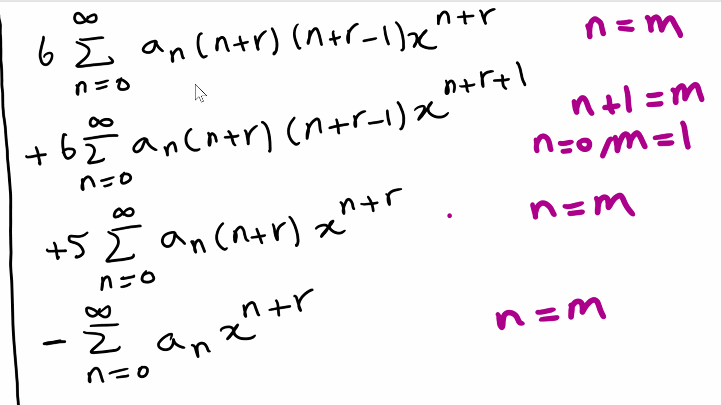
\includegraphics[width = 0.95 \textwidth]{image4.png}

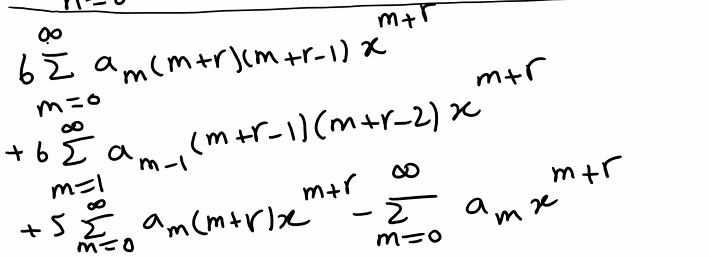
\includegraphics[width = 0.95 \textwidth]{image5.png}

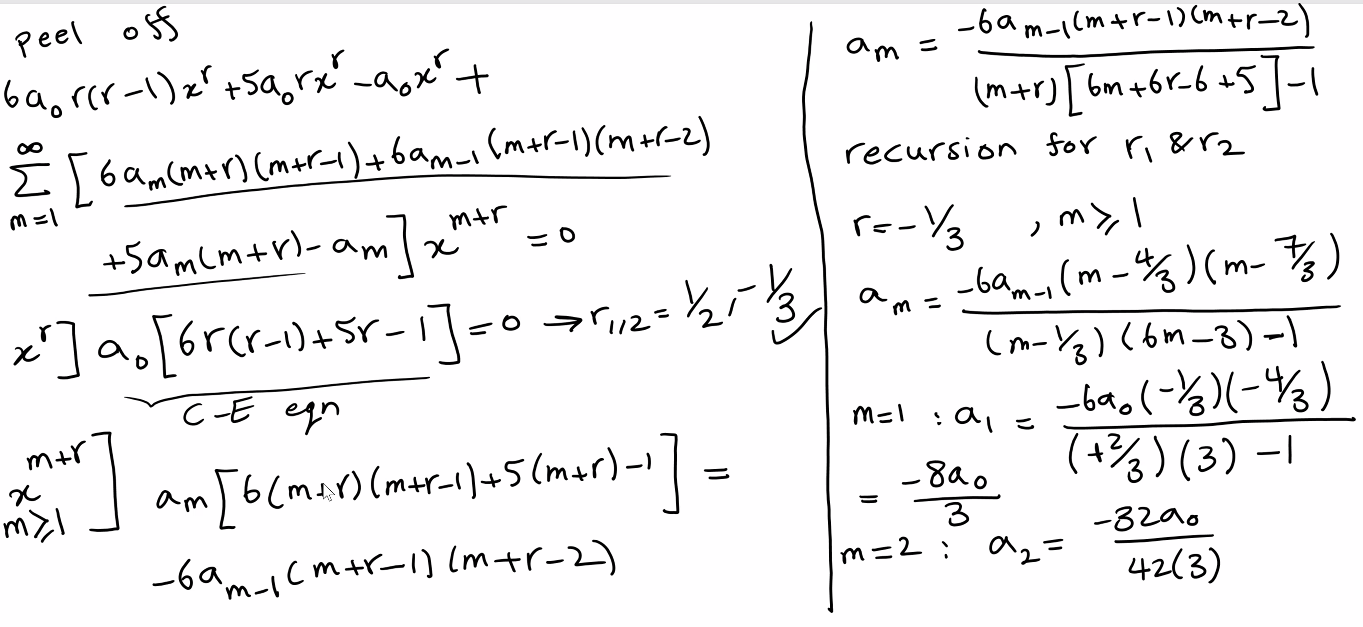
\includegraphics[width = 0.95 \textwidth]{image6.png}

$$y_1(x) = a_0 x^{\frac{-1}{3}} \left[ 1- \frac{8}{3} x - \frac{32}{3(42)} x^2 + ... \right]$$

$r = \frac{1}{2}$: If we follow the same steps, we get 

$y_2(x) = \underbrace{a_0}_{\text{A different } a_0} x^{\frac{1}{2}} \left[ 1 + \frac{3}{22} x - \frac{22}{22.68}x^2 + ... \right]$

Hence the general solution is $y = C_1 y_1 (x) + C_2 y_2 (x)$

\subsubsection{Convergence: ratio test}

$$\sum_{m = 0}^\infty C_m: \lim_{m \to \infty} | \frac{C_{m+1}}{C_m} | < 1$$

$$y(x) = \sum_{m = 0}^\infty a_m x^{m+r}$$

Ratio test:

$$\lim_{m \to \infty} | \frac{a_{m+1} x^{m+r+1}}{a_m x^{m+r}} | = |x| \lim_{m \to \infty} | \frac{a_{m=1}}{a_m}$$

For this example:

$$ |x| \lim_{m \to \infty} | \frac{a_{m=1}}{a_m}, a_m = \frac{-6 a_{m-1} (m+r-1) (m+r-2)}{(m+r) (6m + 6r - 1) - 1}$$

$$ |x| \lim_{m \to \infty}  \frac{-6 a_{m-1} (m+r-1) (m+r-2)}{(m+r) (6m + 6r - 1) - 1} = |x| \cdot 1$$

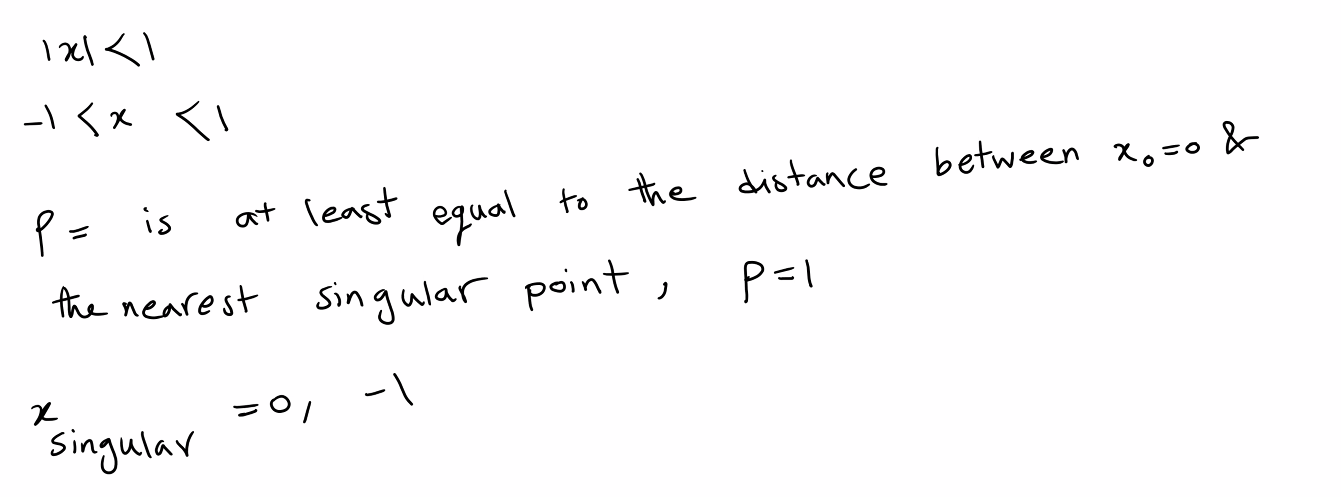
\includegraphics[width = 0.95 \textwidth]{image7.png}